%%==================================================
%% chapter01.tex for BIT Master Thesis
%% modified by yang yating
%% version: 0.1
%% last update: Dec 25th, 2016
%%==================================================
\chapter{ReL4系统设计}
\label{chap:ReL4_intro}
ReL4是一款用Rust编写的,兼容seL4基本系统调用的高性能异步微内核,它借鉴了seL4的权限管理、内存管理和SMP设计等基本框架,但在IPC机制和任务调度方面进行了优化和改进,如\ref{fig:ReL4_framework}所示,ReL4将IPC从内核中移除,内核仅支持基于硬件的通知机制,应用程序仅需在注册时陷入内核分配相应的硬件资源,在通知过程中,通过硬件直接传递信号,减少特权级切换;同时,ReL4在用户态设计了一套异步运行时,由用户态实现异步IPC和异步系统调用,所有的数据传递都通过共享缓冲区实现,由通知机制进行同步,并提供协程的概念作为任务调度的基本单位,提升系统并发性;最后,ReL4使用TAIC——一种基于用户态中断的调度器硬件加速单元,减少低并发场景下的运行时开销。

\begin{figure*}[htbp]
  \centering
  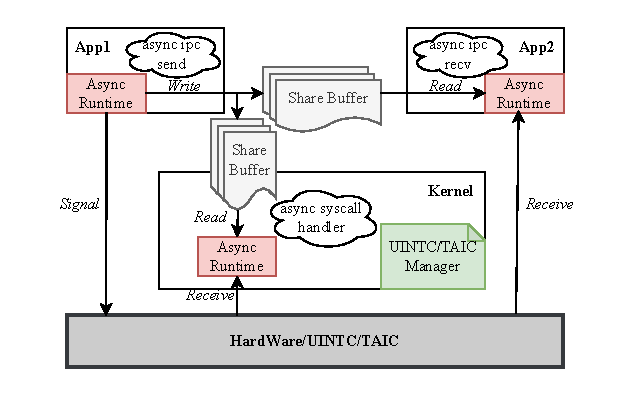
\includegraphics{figures/ReL4_framework.drawio.pdf}
  \caption{ReL4的系统架构图}\label{fig:ReL4_framework}
\end{figure*}

ReL4的设计原则如下:
\begin{itemize}
  \item 内核最小化原则:精简内核,在内核中移除同步IPC,由用户态实现。
  \item 避免特权级切换:通过软硬结合等手段避免系统在IPC、通知和系统调用过程中的频繁地进行特权级切换。
  \item 易用性原则:通过编程语言支持和接口封装等手段,避免用户层接口的改动,同时提供更易用的异步化接口简化编程模型。
\end{itemize}

本章的剩余内容将详细介绍系统设计的两个核心内容:通知机制和异步运行时。
\section{通知机制}

ReL4将整个系统中的通知机制按照收发双方的特权级进行分类:1)用户态通知用户态;2)内核态通知用户态;3)用户态通知内核态;4)内核态通知内核态。本文希望借助用户态中断并辅助软件设计,尽量避免通知过程中的特权级切换。对于1)和2)而言,ReL4借助用户态中断,重新设计了seL4的通知机制,避免了特权级切换,对于3),ReL4通过系统调用的形式通知内核,并通过自适应轮询机制减少通知的次数,对于4),不存在特权级的切换,仅通过核间中断就可以实现内核态之间的通知。因此本文将着重介绍基于用户态中断的通知机制(U-notification),以及用于减少通知次数的自适应混合轮询机制。

\subsection{U-notification}
如\ref{fig:u-notification}所示,用户态中断使得控制流和数据流相互分离。ReL4在notification内核对象中维护了对应的硬件资源索引,控制流主要由用户态向内核进行注册,申请硬件资源,数据流则通过特殊的用户态指令访问用户态中断控制器,从而在通信过程中避免了特权级的切换。

\begin{figure*}[htbp]
  \centering
  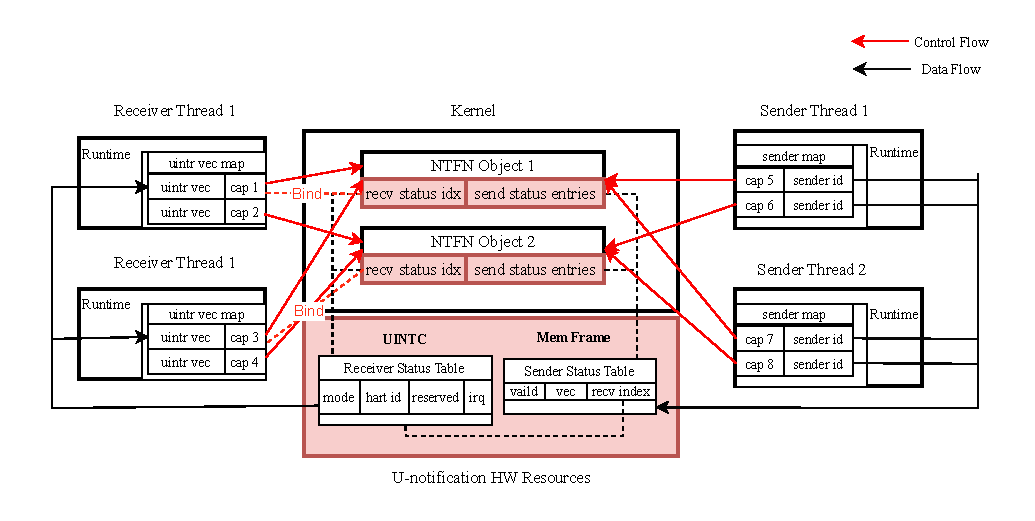
\includegraphics[width=0.9\textwidth]{figures/uintr_for_ntfn.drawio.pdf}
  \caption{ReL4的系统架构图}\label{fig:u-notification}
\end{figure*}

控制流主要分为发送方的注册和接收方的注册。接收方在用户态通过$Untyped\_Retype$。申请一个Notification对象之后,调用$TCB\_Bind$接口进行硬件资源绑定,运行时进一步调用$UintrRegisterReceiver$系统调用,将运行时中定义的用户态中断向量表注册到TCB中,申请UINTC的接收状态表项,并绑定到Notification对象及其对应的线程上。发送方通过Capability派生的形式(直接构造发送方的Capability空间,或通过内核转发的形式获取Capability)获取指向Notification对象的Capability,第一次调用Send操作时,运行时会判断Cap是否有对应的Sender ID,如果没有,则调用$UintrRegisterSender$系统调用进行发送端注册,并填充对应的SenderID。相关资源的回收则通过已有的$revoke$或$delete$系统调用注销内核对象。

数据流由硬件直接传递,无需通过内核。发送端在注册完成之后,可以直接调用$uipi\_send$指令,指令根据Sender Status Table Entry中的索引设置中断控制器中的寄存器。如果接收端本身在CPU核心上运行,会立刻被中断并跳转到注册的中断向量表,否则会等到被内核重新调度时再处理通知。

\subsection{自适应的混合轮询}
虽然用户态中断的开销小于特权级切换,但仍然对程序局部性和内存局部性不够友好,且用户态通知内核态仍然要进行特权级的切换,而轮询虽然可以避免中断式通知,但却会导致CPU资源的浪费,因此ReL4在共享缓冲区中维护通知处理程序的就绪状态标识。当通知频率足够高或处理程序负载足够大,以至于上一个通知还未被处理完成,下一个通知就即将发起,处理程序会始终处于运行状态,此时发送端无需发送额外的通知,其工作方式等价于轮询模式。当通知频率较低时,处理程序在大部分时间处于阻塞状态,节省CPU资源,工作方式等价于中断模式。

\section{异步运行时}
由于内核不再支持同步IPC,为了提升用户态的易用性,ReL4在用户态设计了异步运行时,它提供了如下功能,使得用户态程序设计变得更加简单和高效:
\begin{itemize}
  \item 共享缓冲区:用于跨进程的零拷贝数据传递。
  \item 协程与调度器:提升用户态的并发度,减少用户态中断和特权级切换次数,并为不同负载的任务提供可定制性调度策略。
  \item API兼容层:提供与seL4相同的通知机制、异步系统调用和异步IPC的用户态接口,提升系统易用性。
\end{itemize}

\subsection{共享缓冲区}
由于U-notification只能传递通知信号,因此ReL4依然需要共享缓冲区来作为IPC数据传递的主要形式。以IPC中最常见的Call为例,客户端需要将请求数据准备好并写入共享缓冲区中,而服务端将在某个时刻从共享缓冲区中读取请求,处理后将响应写回共享缓冲区,而客户端也将在之后的某一时刻从共享缓冲区中读取响应并进行相应处理。这个流程中有几个挑战需要明确:
\begin{enumerate}
  \item 请求和响应的格式和长度如何设计才能使得缓冲区访问效率更高。
  \item 在共享缓冲区中如何组织请求和响应的存取形式,才能在数据安全读写的前提下保证性能。
  \item 客户端和服务端如何选择合适的时机来接收数据。
\end{enumerate}

如\ref{fig:ipcitem}所示,一个IPC消息(请求或响应)被定义为 IPCItem,它是IPC传递消息的基本单元,为了减少消息读写以及编解码的成本,ReL4采用定长的消息字段。每个IPCItem的长度被定义为缓存行的整数倍并对齐,消息中的前四个字节存储发送端的sender id,方便后续发送U-notificaiton进行唤醒,后四个字节记录写入的协程id,便于后续进一步唤醒, msg info 用于存储消息的元数据,包含了消息类型、长度等。extend msg 将被具体的应用程序根据不同的用户进行定义。

\begin{figure*}[htbp]
  \centering
  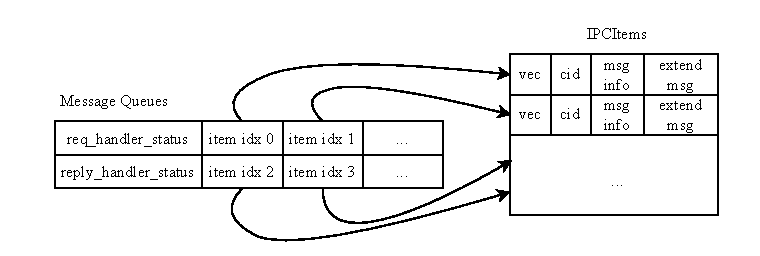
\includegraphics[width=0.9\textwidth]{figures/IPCItem.drawio.pdf}
  \caption{共享缓冲区的结构图}\label{fig:ipcitem}
\end{figure*}

客户端在发起请求之前需要先从缓冲区中申请一个IPCItem并将对应的索引写入请求队列,服务端会根据请求队列中的索引读取请求消息,并将响应写回到对应的IPCItem,并将索引写入响应队列。由于请求队列和相应队列会被一个以上的线程同时访问,因此需要设计同步互斥操作来保证数据的读写安全。同时队列的访问极为频繁,需要尽可能避免数据竞争来保证读写性能。ReL4将请求和响应的索引放到不同的环形队列中,同时不同的发送方和接收方使用不同的环形队列以保证单生产者单消费者的约束,消除过多的数据竞争,最后,ReL4使用无锁的方式[27]进一步提升环形队列的读写性能。

最后,为了支持2.1.2中所提到的自适应轮询机制,ReL4还在队列中维护了对端处理程序的就绪状态标识handler\_status,客户端和服务端将根据该标志位来决定是否发送U-notificaiton。

\subsection{协程与调度器}
传统微内核中的同步IPC会导致发送端线程阻塞,从而造成一些没有依赖的IPC被迫以顺序的形式执行,或者强制要求多线程来实现并发。而ReL4中的异步运行时将协程作为任务的执行单元,以提升用户态并发度。同时,为了减少调度的开销,主要是跨进程唤醒协程的开销,ReL4基于TAIC来进行硬件加速。

如\ref{fig:executor}所示,TAIC是一个基于用户态中断的调度器加速单元,它将用户态中断的中断号与协程号进行一一绑定,并使用硬件来自动唤醒协程。在理想情况下,软件无需手动唤醒协程,然而由于硬件资源有限,用户态中断号仅支持0~31,而协程的数量远远大于这个量级,因此每个运行时中常驻了一个dispatcher协程,并绑定0号中断向量,当中断号不够用时,硬件唤醒对应的dispatcher协程,之后由dispatcher协程手动唤醒其他协程。

\begin{figure*}[htbp]
  \centering
  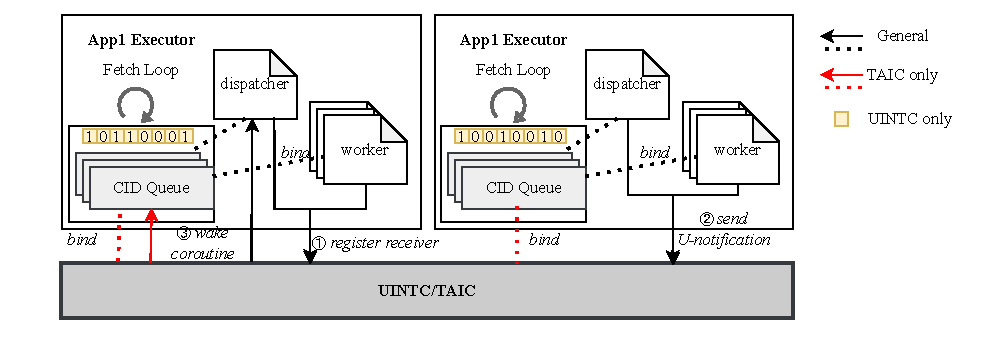
\includegraphics[width=0.9\textwidth]{figures/TAIC.drawio.pdf}
  \caption{调度器的结构图}\label{fig:executor}
\end{figure*}

ReL4将协程分为worker协程和dispatcher协程,用户态的IPC任务都将被封装到worker协程,由运行时内的调度器进行调度,而dispatcher协程则在硬件资源有限的情况下进行二级唤醒。从调度器的角度来看,不同进程的调度器相互独立,每个进程中的 worker协程和dispatcher协程存在着一定的依赖关系。以IPC场景下的客户端为例,worker协程用于发起IPC请求,dispatcher协程则是处理响应。从高吞吐率的角度来讲,自然是希望更快的处理worker协程,而从低延迟的角度来讲则是希望优先调度dispatcher协程,高吞吐和低延迟的特性由上层业务决定,框架层只根据业务配置进行支持。此外,不同的worker协程也需要有轻重缓急之分,以便更有效率地利用CPU资源。

基于上述原因,ReL4在调度器中维护了一个优先级队列,每个协程都被设有相应的优先级,调度器在内部维护了一个优先级位图和若干任务队列,调度器将根据优先级位图选出最高的优先级,找到对应的任务队列并以先进先出的形式选出任务来运行。用户态程序根据业务特点设置相关的优先级,以达到性能调优的目的。

\subsection{API兼容层}

为了使异步系统调用和异步IPC能够与同步接口保持一致,异步运行时提供了异步系统调用和IPC的的hook库,用户态的请求将会被hook库接管,hook库根据不同的调用类型,来自动选择是否转化为异步系统调用或IPC。需要注意的是,无法转化为异步系统调用的主要有以下两类:
\begin{enumerate}
  \item 由于异步系统调用依赖于异步运行时,因此与异步运行时初始化相关的系统调用无法被异步化。
  \item 对于实时性要求较高的系统调用无法进行异步化,如$get\_clock()$。
\end{enumerate}

而为了尽可能兼容seL4中的capability机制,运行时库中还维护了notification cap与用户态中断相关资源的映射:
\begin{enumerate}
  \item sender map:由于U-notification以及异步IPC都无需通过内核,因此运行时需要维护capability与sender id以及共享缓冲区的映射关系。
  \item uintr vec map:用户态中断通过中断向量区分发送端,而seL4通过capability区分发送端,为了兼容多发送端,运行时需要维护相关的映射关系。
\end{enumerate}

